\section{Minimalizacja form boolowskich}
Naukę minimalizacji funkcji logicznych najlepiej zacząć od praktycznego przykładu.

\subsubsection*{System zabezpieczenia pracy robota}
Problem: Mamy robota, który posiada 4 przełączniki bezpieczeństwa: A, B, C i D. Robot ma działać (wyjście układu ma wynosić 1), kiedy co najmniej dwa przełączniki obok siebie są wciśnięte (mają stan 1).\\

Najpierw rozpisujemy tabelę prawdy układu, czyli zależność wyjścia od wejścia. Określa ona, jaka ma być odpowiedź naszego systemu na konkretne stany podawane na jego wejście. Rozpisujemy więc wszystkie opcje stanów:

\begin{table}[h]
    \centering
    \begin{tabular}{|c|c|}
        A B C D (liczba w dziesiętnym) & Y (wyjście)\\
        \hline
        0 0 0 0 (0) & 0 \\
        0 0 0 1 (1) & 0 \\
        0 0 1 0 (2) & 0 \\
        0 0 1 1 (3) & 1 \\
        0 1 0 0 (4) & 0 \\
        0 1 0 1 (5) & 0 \\
        0 1 1 0 (6) & 1 \\
        0 1 1 1 (7) & 1 \\
        1 0 0 0 (8) & 0 \\
        1 0 0 1 (9) & 0 \\
        1 0 1 0 (10) & 0 \\
        1 0 1 1 (11) & 1 \\
        1 1 0 0 (12) & 1 \\
        1 1 0 1 (13) & 1 \\
        1 1 1 0 (14) & 1 \\
        1 1 1 1 (15) & 1 \\
        \hline
    \end{tabular}
\end{table}

Teraz mamy tak na prawdę zdefiniowaną funkcję, którą moglibyśmy zapisać jako:\\
$$Y = \Sigma(3,6,7,11,12,13,14,15)$$
poprzez zapisanie w nawiasie wszystkich liczb, dla których wyjście naszego układu wynosi 1. Równanie takiej funkcji wyglądałoby następująco:
$$Y = \bar{A}\bar{B}CD + \bar{A}BC\bar{D} + \bar{A}BCD + A\bar{B}CD + AB\bar{C}\bar{D} + AB\bar{C}D + ABC\bar{D} + ABCD$$
Czy ta funkcja jest jednak najprostszym zapisem umożliwiajacym zrealizowanie układu? W tym przypadku od razu widać że, przykładowo, kiedy A i B są jedynkami nie mają znaczenia wartości B i C, układ i tak będzie podawał na wyjście 1. Możemy to jednak sprawdzić również algorytmicznie, wykorzystując do tego \textbf{metodę Karnaugh}.\\

W tym celu formujemy tabelę Karnaugh. Jest to tak na prawdę tabela prawdy, zapisana w delikatnie inny sposób. Tabela \textbf{musi} być zakodowana \textbf{w kodzie Gray'a}. W komórkach tabeli umieszczamy wartość wyjścia $Y$ dla danej kombinacji wejść A B C i D. W prawym górnym rogu dla wygody umieszczamy zapis liczby w systemie dziesiętnym, której odpowiada dana kombinacja wejść.

\begin{table}[h]
    \centering
    \begin{tabular}{|l|c|c|c|c|} \hline
        \diagbox[width=4em]{A B}{C D}
        & 0 0 & 0 1 & 1 1 & 1 0\\
        \hline
        0 0 & 0 \textsuperscript{0}& 0 \textsuperscript{1} & 1 \textsuperscript{3} & 0 \textsuperscript{2} \\
        0 1 & 0 \textsuperscript{4}  & 0 \textsuperscript{5}  & 1 \textsuperscript{7} & 1 \textsuperscript{6} \\
        1 1 & 1 \textsuperscript{12} & 1 \textsuperscript{13} & 1 \textsuperscript{15} & 1 \textsuperscript{14} \\
        1 0 & 0 \textsuperscript{8}  & 0 \textsuperscript{9}& 1 \textsuperscript{11}  & 0 \textsuperscript{10} \\
        \hline
    \end{tabular}
\end{table}

Po zapisaniu tablicy przystępujemy do grupowania jedynek (w przypadku realizacji układu na bramkach NAND) lub zer (w przypadku zastosowania bramek NOR). Zasady grupowania w obu przypadkach są takie same. Grupujemy jedynki w grupy o wielkości kolejnych potęg dwójki, przy czym zależy nam na utworzeniu \textbf{jak największych grup}. Możemy grupować jedynki poziomo lub pionowo (nie po ukosie!). Grupy muszą być symetryczne względem tabeli, natomiast elementy grupy \textbf{nie muszą ze sobą bezpośrednio sąsiadować}. Wszystkie jedynki muszą zostać zgrupowane! Grupy mogą na siebie nachodzić (jedna jedynka może być w wielu grupach jednocześnie). W powyższym przykładzie możemy zgrupować pozycje: 12, 13, 15, 14; 3, 7, 15, 11; 7, 6, 15, 14. Powstają więc trzy grupy.

\begin{center}
    \begin{karnaugh-map}[4][4][1][$D$][$C$][$B$][$A$]
    \minterms{3,6,7,11,12,13,14,15}
    \autoterms[0]
    \implicant{12}{14}
    \implicant{3}{11}
    \implicant{7}{14}
    \end{karnaugh-map}
\end{center}

Postać optymalną funkcji odczytujemy zapisując równanie na podstawie grup, które właśnie utworzyliśmy. W tym celu patrzymy na pierwszą grupę (12, 13, 15, 14) i sprawdzamy \textbf{które zmienne ulegają zmianie wartości na całej przestrzeni grupy}. W tym przypadku, A i B dla całej grupy wynoszą 1 i 1, a C i D zmieniają wartości. A i B są więc niezmienne w całej grupie, więc gdy powiemy "jedynki są we wszystkich komórkach, gdzie A i B wynosi 1" jednoznacznie zidentyfikujemy ten wiersz jedynek. Odpowiada to zapisowi w ZNPS $Y = AB$. To równanie daje 1 tylko gdy obie wartości A i B wynoszą 1. Kolejna grupa to pionowa grupa 3, 7, 15, 11. Zmienne nie ulegające zmianie w tej grupie to C i D, więc nasze równanie rozszerza się do $Y = AB + CD$. W ostatniej grupie 7, 6, 15, 14 niezmienne są B i C, więc finalna postać naszego równania to:
$$Y = AB + CD + BC$$
Ta postać jest dużo prostsza niż postać przed minimalizacją. Algorytm "zauważył", że wystarczy zsumować iloczyny wszystkich kombinacji sąsiadujących ze sobą przycisków, aby dotrzeć do najprostszej formy rozwiązania problemu. Możemy sprawdzić, że dla wszystkich wejść z tabeli prawdy, to równanie daje taki sam rezultat jaki przewiduje ta tabela.

Skoro już zminimalizowaliśmy funkcję, pokażmy co tak na prawdę nam to dało. Dokonajmy \textbf{syntezy} naszego układu na bramkach logicznych, tzn. narysujmy schemat faktycznego, fizycznego układu realizującego te funkcje. W celu wizualizacji wykorzystamy applet Falstad dostępny na https://www.falstad.com/circuit/. Synteza układu zapisanego w ZNPS (minimalizacja po jedynkach, suma iloczynów) polega na narysowaniu układu w postaci \textbf{dwóch warstw} bramek logicznych \textbf{NAND}. Na początek rysujemy po lewej stronie linie przewodów odpowiadających wejściom układu. Do nich będziemy podłączać nasze bramki logiczne. Następnie rysujemy pierwszą warstwę bramek NAND. Bramek będzie tyle, ile mamy \textbf{iloczynów} w równaniu opisującym funkcje. Każdemu iloczynowi odpowiada jedna bramka NAND o tylu wejściach, ile czynników jest w iloczynie. W naszym przypadku będą to trzy bramki NAND o dwóch wejściach każda. Do wejść każdego z NANDów podłączamy zmienne, z których składa się dany iloczyn. Jeśli zmienna jest zanegowana, należy ją podłączyć przez negator. Kiedy podłączymy wszystkie bramki warstwy pierwszej należy podłączyć warstwę drugą. Warstwa druga będzie się składać z jednej bramki NAND, która będzie miała tyle wejść, ile iloczynów mamy w równaniu. W naszym przypadku są to trzy iloczyny, więc też trzy wejścia. Do tego NANDa podłączamy wszystkie wyjścia NANDów z pierwszej warstwy, a jego wyjście stanowi wyjście naszego układu $Y$. Korzystając z symulacji można sprawdzić, że nasz układ działa prawidłowo. Link do symulacji: 

{\tiny https://www.falstad.com/circuit/circuitjs.html?ctz=DwYwlgTgBAZgvAIgIwKgFwM6IAwDpsEECsqYIiSeATAVQOx0DM2AHFQGwCcndqIARoiLZUAB0EIALI1QA3CENQBbTEICmAWiQoAfACgoUYABkoAD0RakVKNZZQrN9pNTwEIgPT7DJ85ee2VPYaAc6uOAheBkamFgha7IHBSIlhsBFRPrGIjDZ2ULlQaW6e3kYA7n7x2nlBDjW27CLp7pFlwJVxIZJJDgFInFThrZkVVQm9E1RE7MOl0R1VhfmFQSxzbQtm49ZIBXT12ERQks0lqBhgiFQu6GqIAIKbPttdTAWJGkQH7LMtzZdrrc0PcEAAhAA6ADtnkZXpZph8HPZGJwNlBAQgbqgQYgAMKw4DwrGMAo9U77dGY7F3RAAEUJxKQqIKxxuPXYJH+FyuWOBoIA6gBDCAYNDlIVQACS0MZSyQKNJ0mwRRk3IxvJpuIQwtF4slUplMNGwAAckKoQATKpISQ9JB0RI3FUOv7nE3mq02u1Qeg2Z2+uhDbkei3WuK2nqMdj2APR9Yh9qdSwNFIqxxQIh2jYm5PIH1p+rWRpnDJJ8b9QZ9KNEYPu8sRgtV7q2QY5hspp0zeqJRgsW71hZ5yO+7tTGbtodLf0sFE2LMDstTxs9NYFGcJwc+PMtxi16uZ7OJ5cUH17my72uT7c7Xv9nuHxcjDv5qP3iZ9p-zHye8M5GiBjYkgpIB6JgFCOSEnmAauuuKrTG6S43nEAZ+nBoHHsh-7wbOvoUvG15jHEwFOkGJySLGQaEUSVR2vB+6SN20xcucGpAjioIAJqbMAHjgBA+hAA}

\begin{figure}[H]
    \centering
    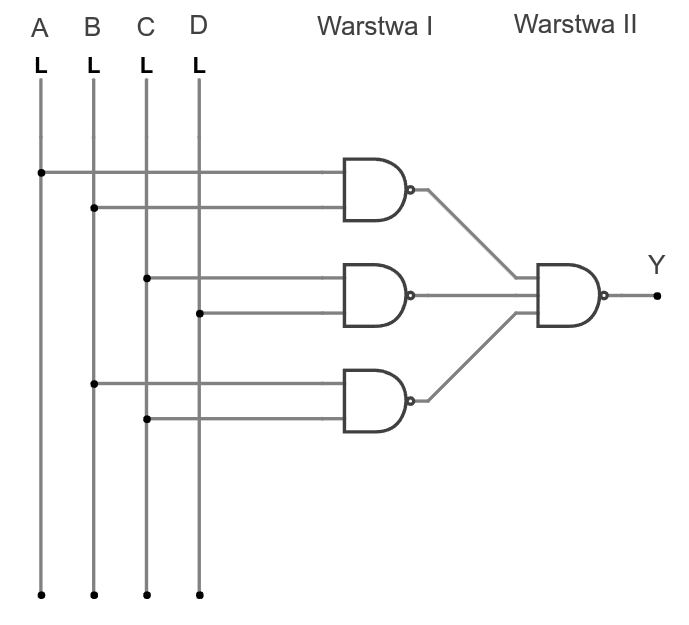
\includegraphics[width=0.7\textwidth]{img/robot_komb_schemat.png}
    \caption{Synteza układu}
\end{figure}

To koniec naszego zadania. Co warto zauważyć, wielkość naszego układu i jego skomplikowanie bezpośrednio wynika ze skomplikowania równania. Minimalizacja pozwala nam więc znacznie ograniczyć ilość elementów w układzie, obniżając jego koszty wykonania.

\subsubsection*{Przykłady minimalizacji}
Przykłady częściowo z książki Technika cyfrowa. Zbiór zadań z rozwiązaniami Jerzy Tyszer, Grzegorz Mrugalski, Artur Pogiel, Dariusz Czysz
\begin{enumerate}
    \item $\Sigma(0-2, 4, 6)$ \\ \begin{karnaugh-map}[4][2][1][$C$][$B$][$A$]
    \minterms{0,1,2,4,6}
    \autoterms[0]
    \implicant{0}{1}
    \implicantedge{0}{4}{2}{6}
    \end{karnaugh-map}
    $Y = \bar{A}\bar{B} + \bar{C}$

    \item $\Sigma(1, 3, 5-7)$ \\ \begin{karnaugh-map}[4][2][1][$C$][$B$][$A$]
    \minterms{1,3,5,6,7}
    \autoterms[0]
    \implicant{1}{7}
    \implicant{7}{6}
    \end{karnaugh-map}
    $Y = AB + C$

    \item $\Sigma(1, 3-7, 9, 11-15)$ \\ \begin{karnaugh-map}[4][4][1][$D$][$C$][$B$][$A$]
    \minterms{1,3,4,5,6,7,9,11,12,13,14,15}
    \autoterms[0]
    \implicant{1}{11}
    \implicant{4}{14}
    \end{karnaugh-map}
    $Y = B+D$

    \item $\Sigma(1, 4-7, 9, 14, 15)$ \\ \begin{karnaugh-map}[4][4][1][$D$][$C$][$B$][$A$]
    \minterms{1,4,5,6,7,9,14,15}
    \autoterms[0]
    \implicant{4}{6}
    \implicant{7}{14}
    \implicantedge{1}{1}{9}{9}
    \end{karnaugh-map}
    $Y = \bar{A}B+BC+\bar{B}\bar{C}D$

    \item $\Sigma(0, 2, 5, 7, 8, 10, 13, 15)$ \\ \begin{karnaugh-map}[4][4][1][$D$][$C$][$B$][$A$]
    \minterms{0,2,5,7,8,10,13,15}
    \autoterms[0]
    \implicant{5}{15}
    \implicantcorner
    \end{karnaugh-map}
    $Y = \bar{A}B+BC+\bar{B}\bar{C}D$

    \item $\Sigma(0, 2, 5, 7, 8, 10, 13, 15)$ \\ \begin{karnaugh-map}[4][4][1][$D$][$C$][$B$][$A$]
    \minterms{0,2,5,7,8,10,13,15}
    \autoterms[0]
    \implicant{5}{15}
    \implicantcorner
    \end{karnaugh-map}
    $Y = \bar{A}B+BC+\bar{B}\bar{C}D$
\end{enumerate}
